\chapter{Rundgang durch den Open Stage-Modus}

Die Benutzung des ctGameStudio beginnt mit dem Login mit seinem persönlichen Benutzeraccount
\ref{login}. Daraufhin wird das Spiel geladen, und das Hauptmenü angezeigt \ref{main-menu}.

\begin{figure}
  \centering
  \label{login}
  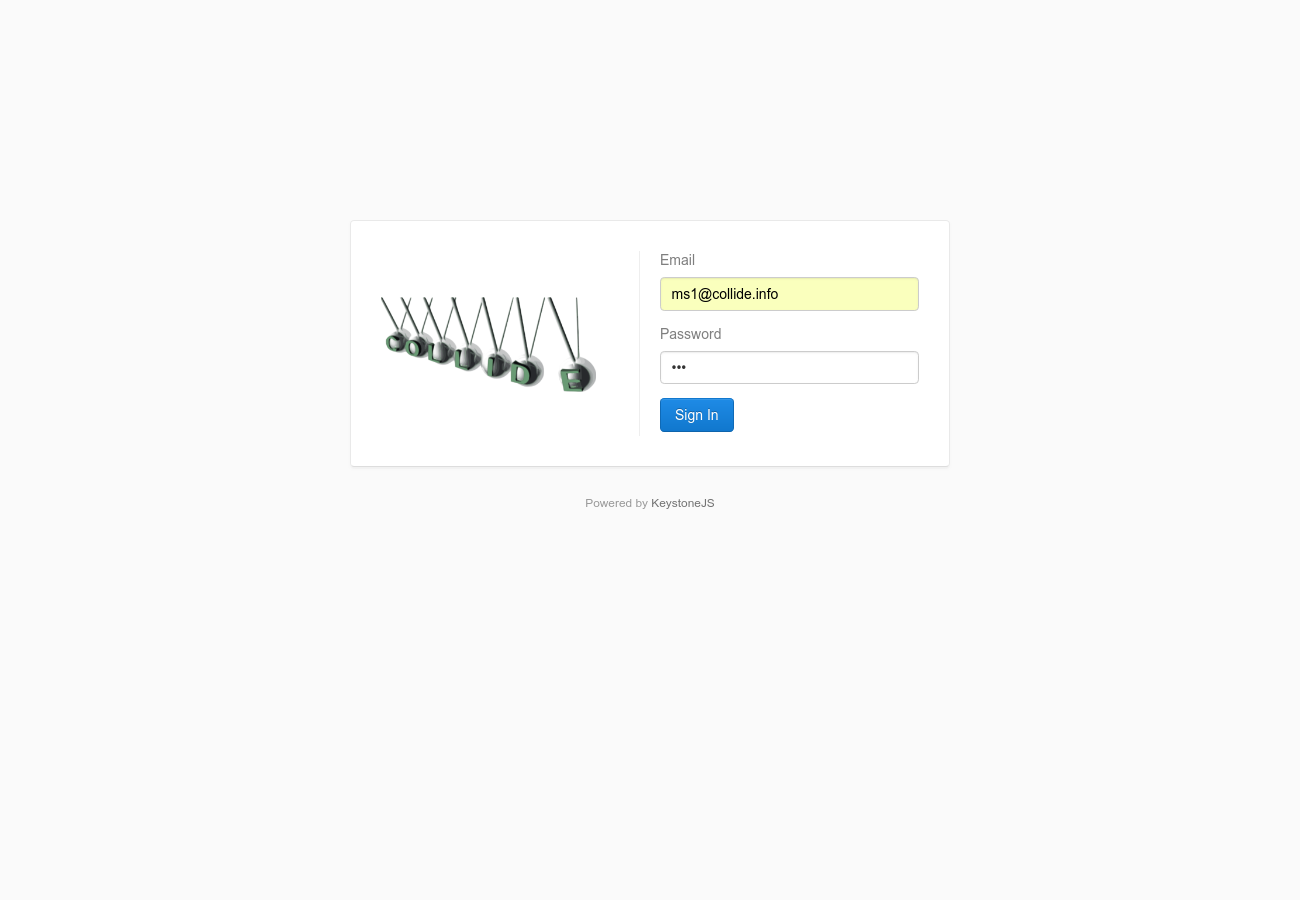
\includegraphics[width=15cm, height=10cm, keepaspectratio]{figures/1-login.png}
  \caption{Der Login-Dialog}
\end{figure}

\begin{figure}
  \centering
  \label{main-menu}
  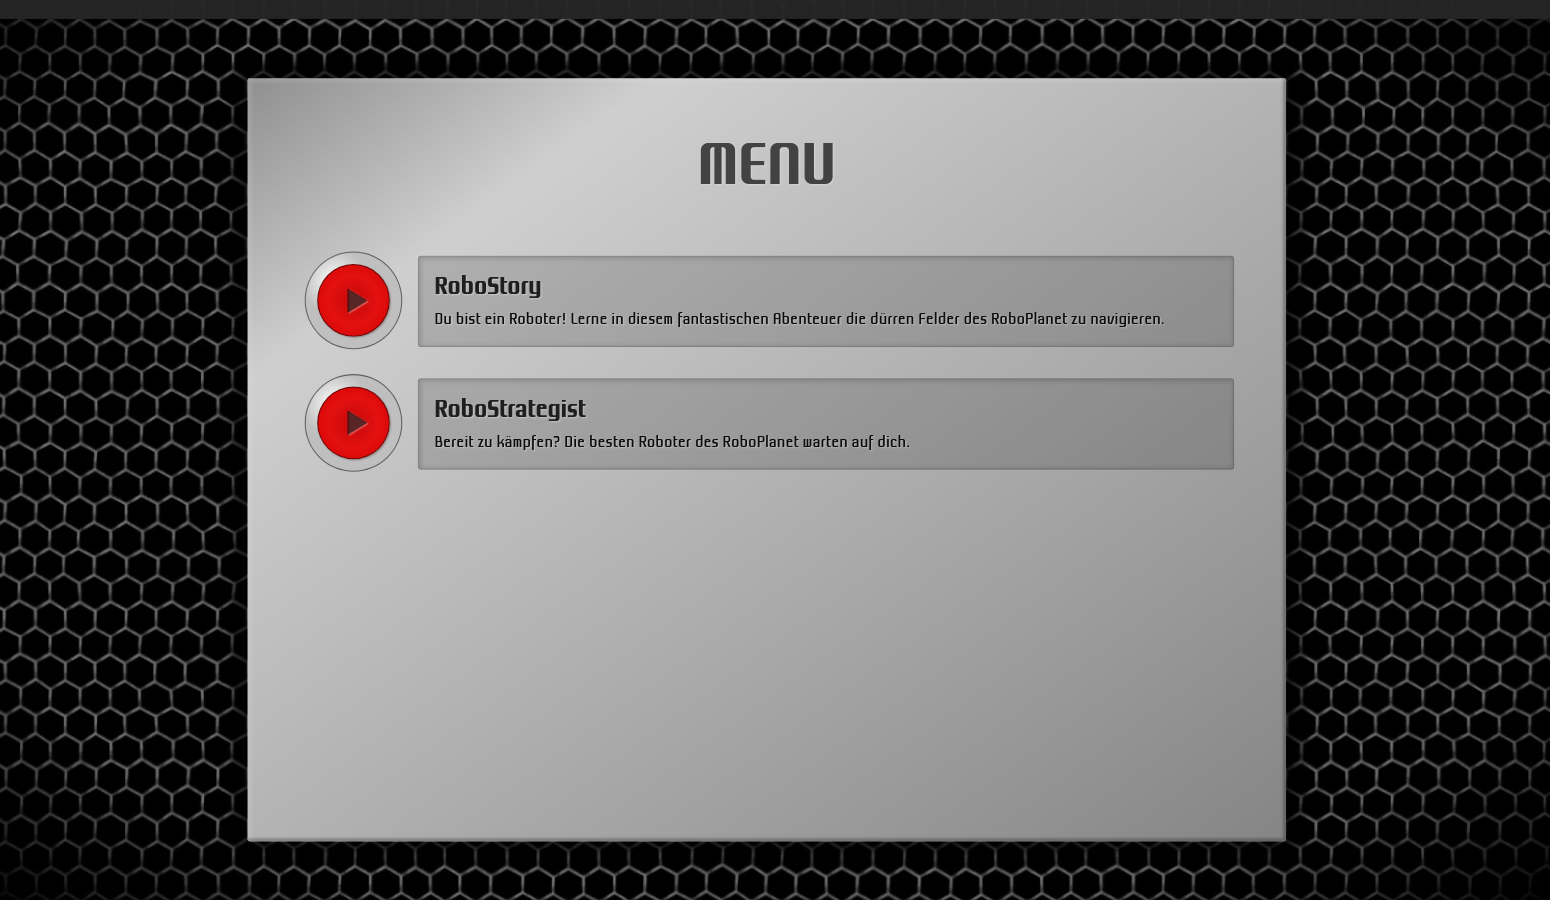
\includegraphics[width=15cm, keepaspectratio]{figures/2-main-menu.png}
  \caption{Das Hauptmenü}
\end{figure}

\begin{figure}
  \centering
  \label{openstage-menu}
  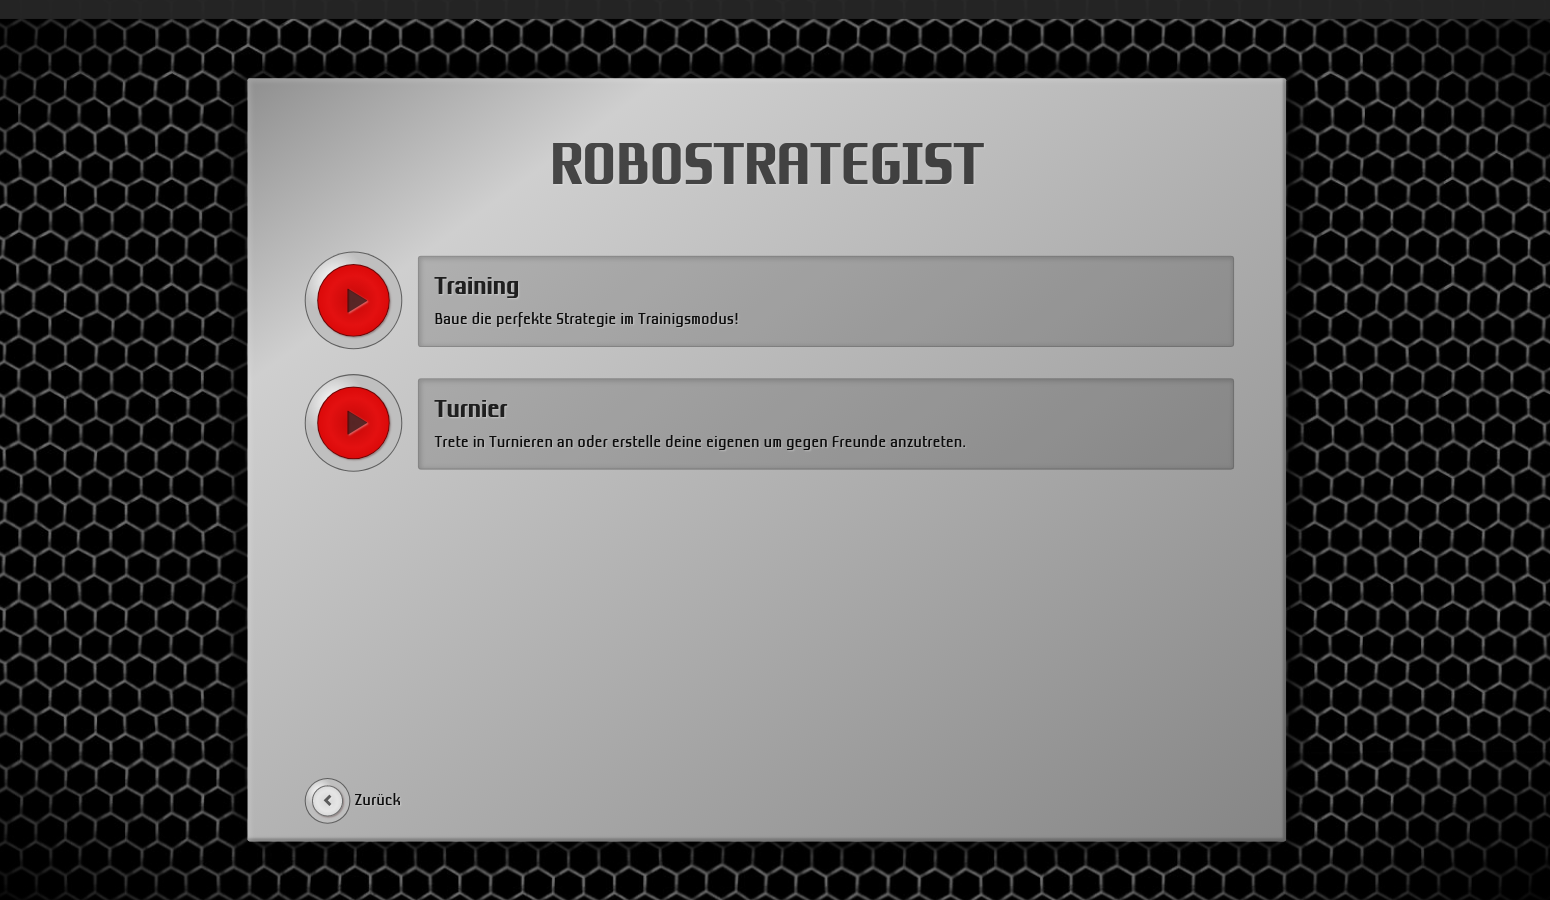
\includegraphics[width=15cm, keepaspectratio]{figures/3-robostrategist-menu.png}
  \caption{Menü des Open Stage-Modus}
\end{figure}

\begin{figure}
  \centering
  \label{training}
  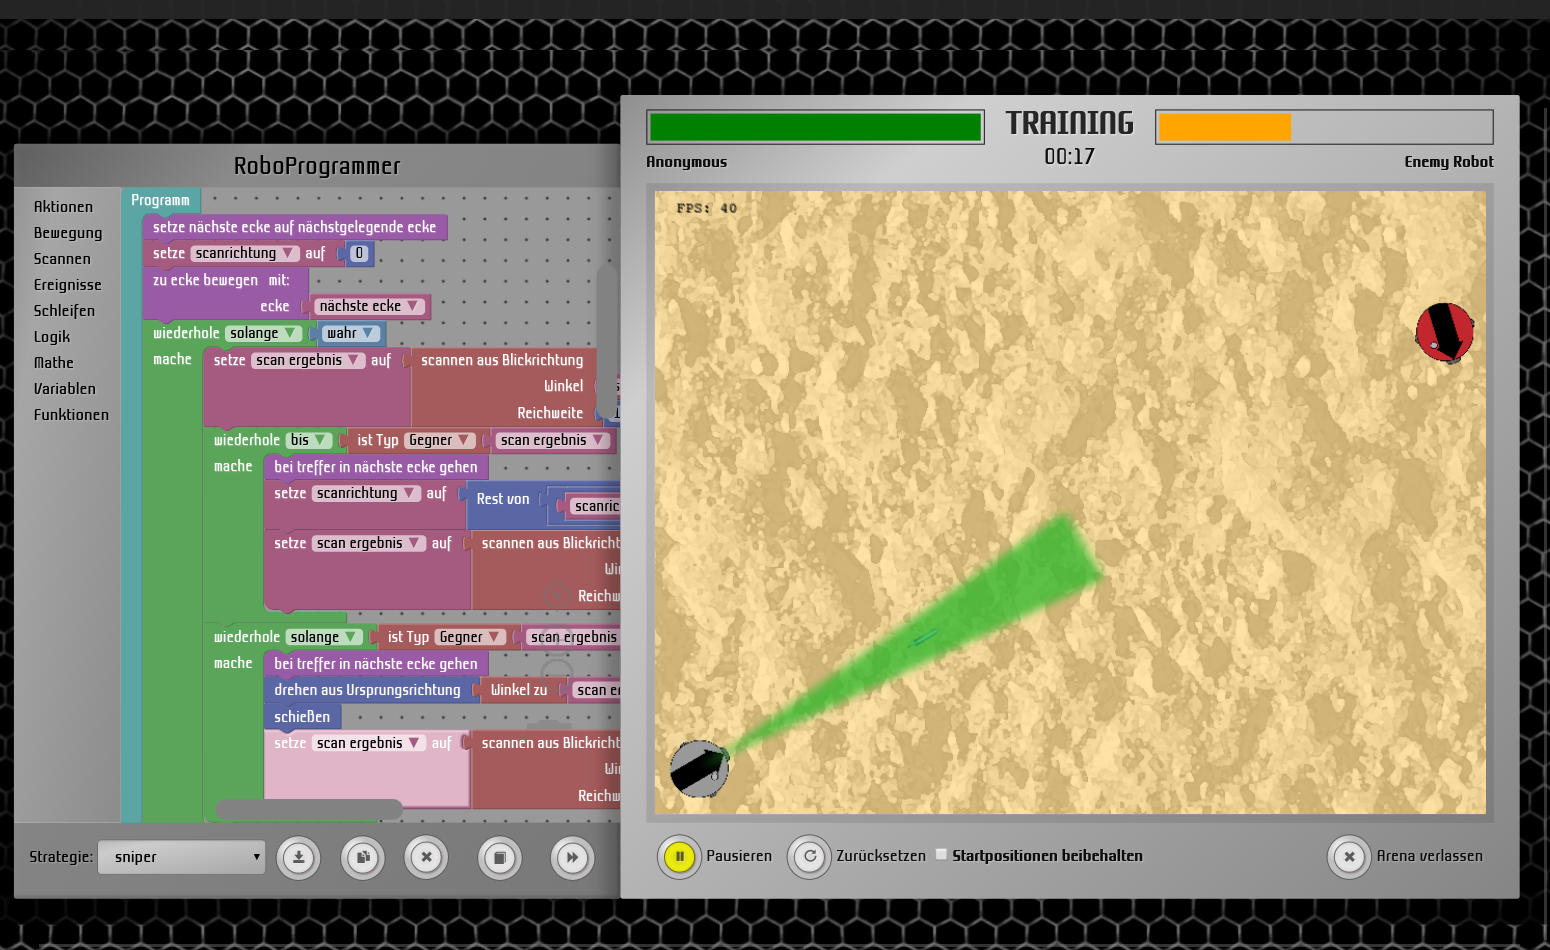
\includegraphics[width=15cm, keepaspectratio]{figures/3-training.png}
  \caption{Die Benutzeroberfläche des Trainings}
\end{figure}

\begin{figure}
  \centering
  \label{training-expanded}
  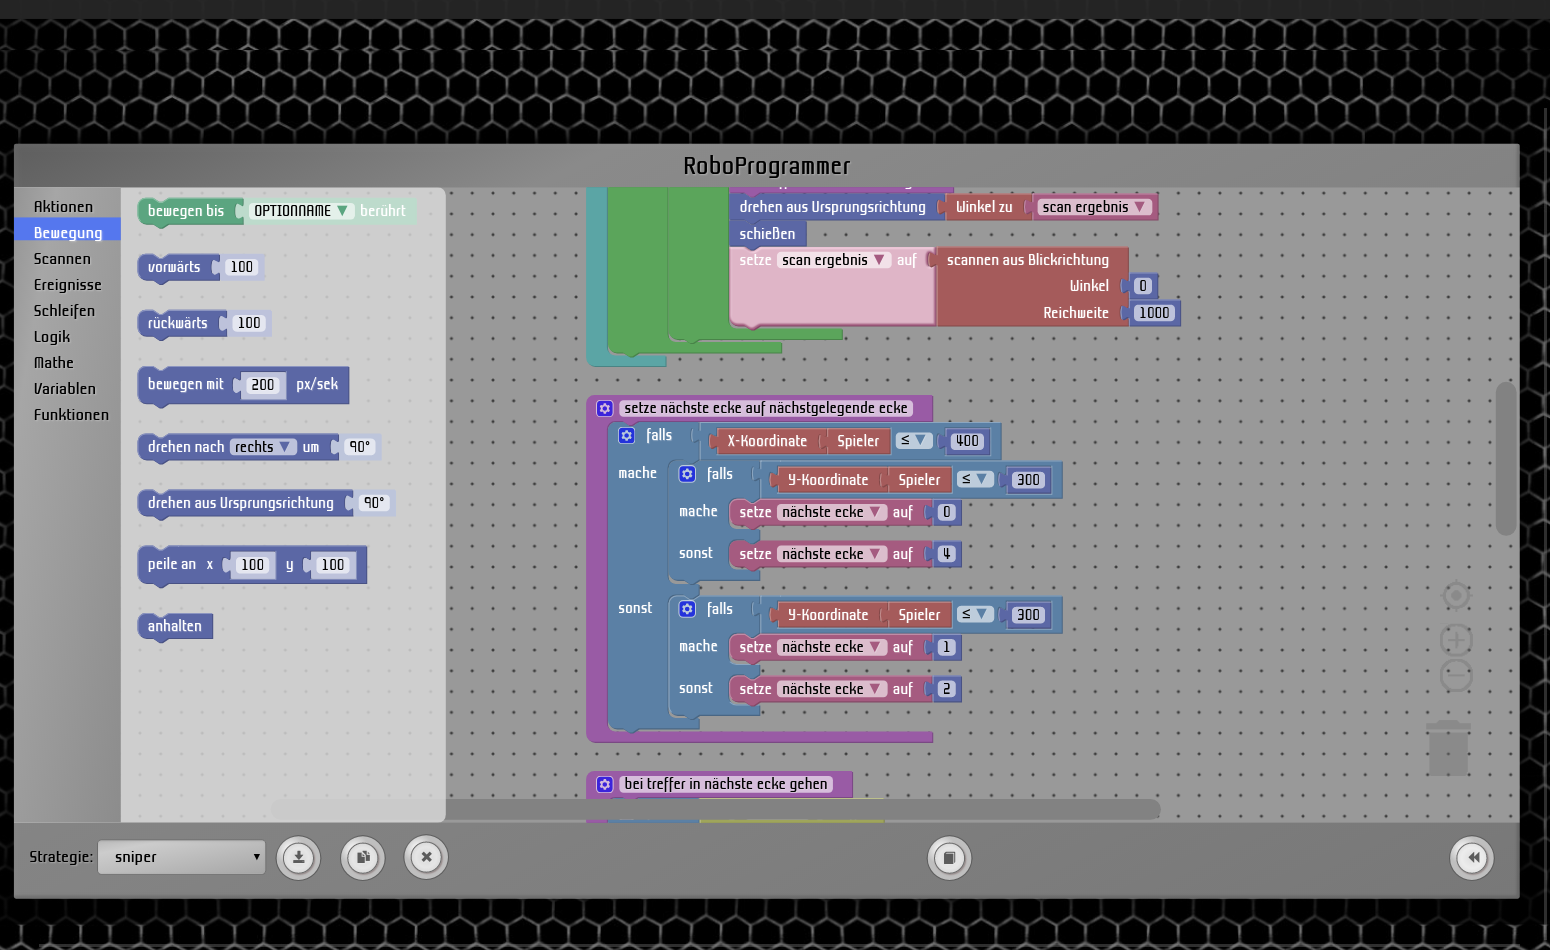
\includegraphics[width=15cm, keepaspectratio]{figures/4-training-expanded.png}
  \caption{Der Strategieeditor im expandiertem Zustand}
\end{figure}

\begin{figure}
  \centering
  \label{tournament-menu}
  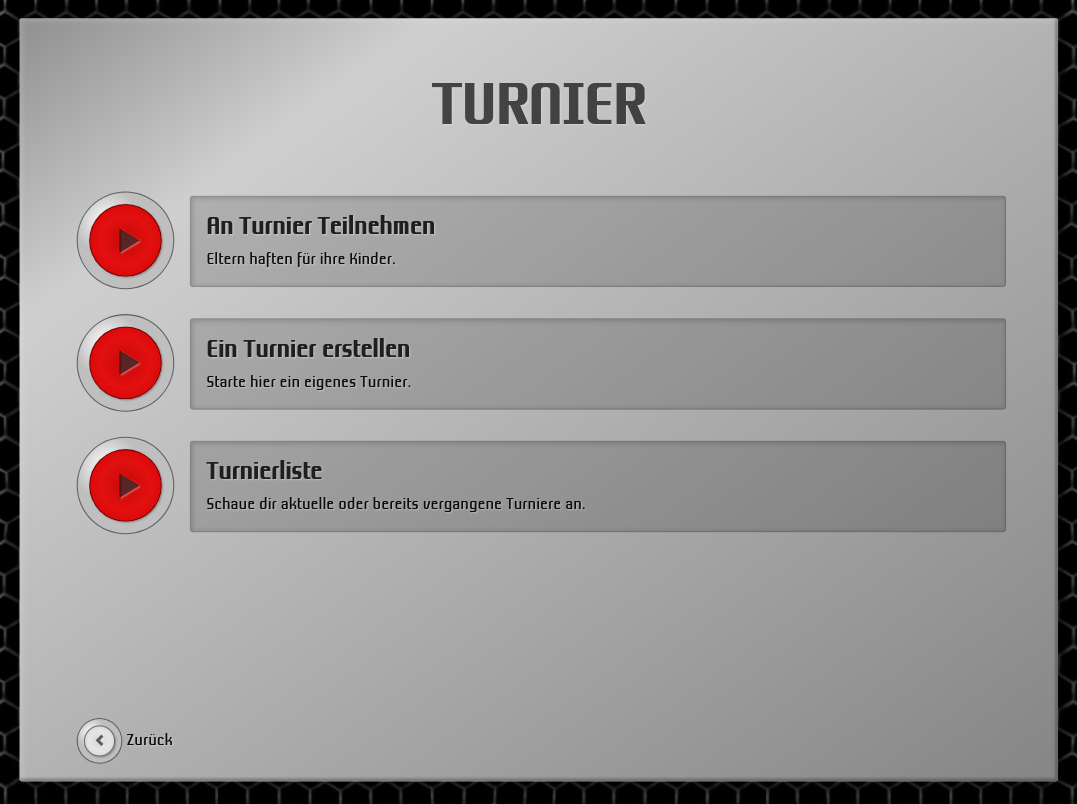
\includegraphics[width=15cm, keepaspectratio]{figures/5-turniermenu.png}
  \caption{Das Turniermenü}
\end{figure}

\begin{figure}
  \centering
  \label{create-tournament}
  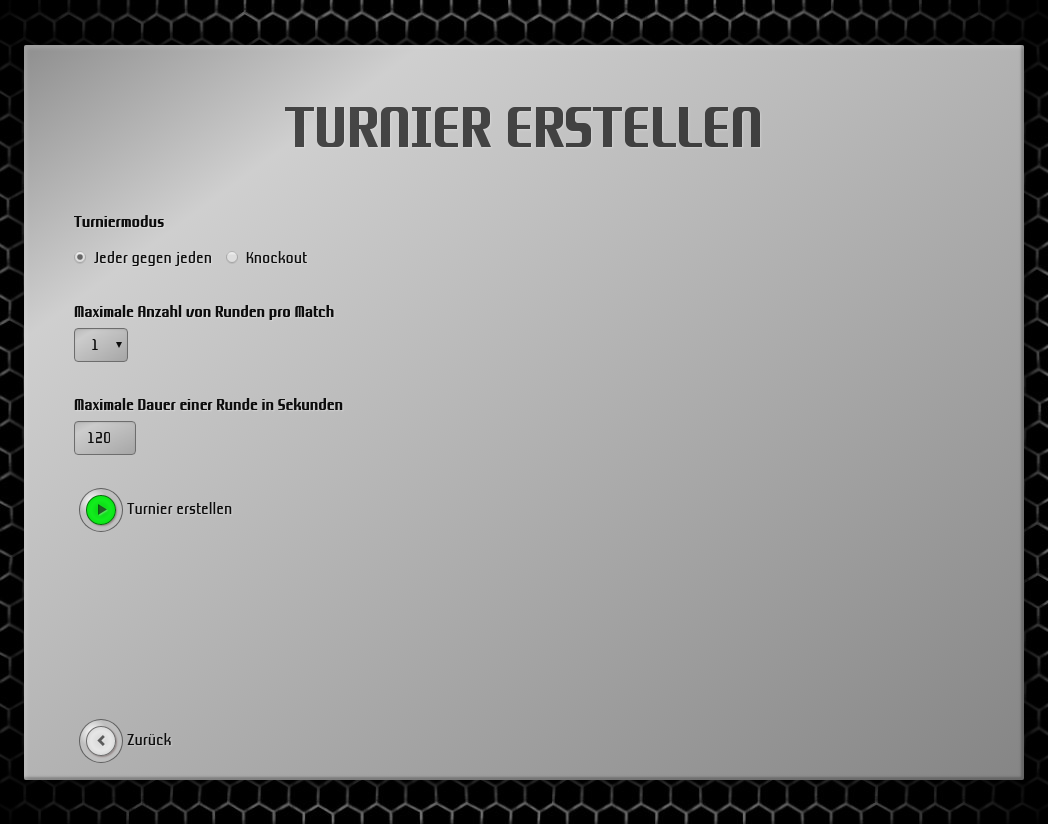
\includegraphics[width=15cm, keepaspectratio]{figures/6-turnier-erstellen-jgj.png}
  \caption{Der Dialog zum Erstellen des Turniers}
\end{figure}

\begin{figure}
  \centering
  \label{create-tournment-code}
  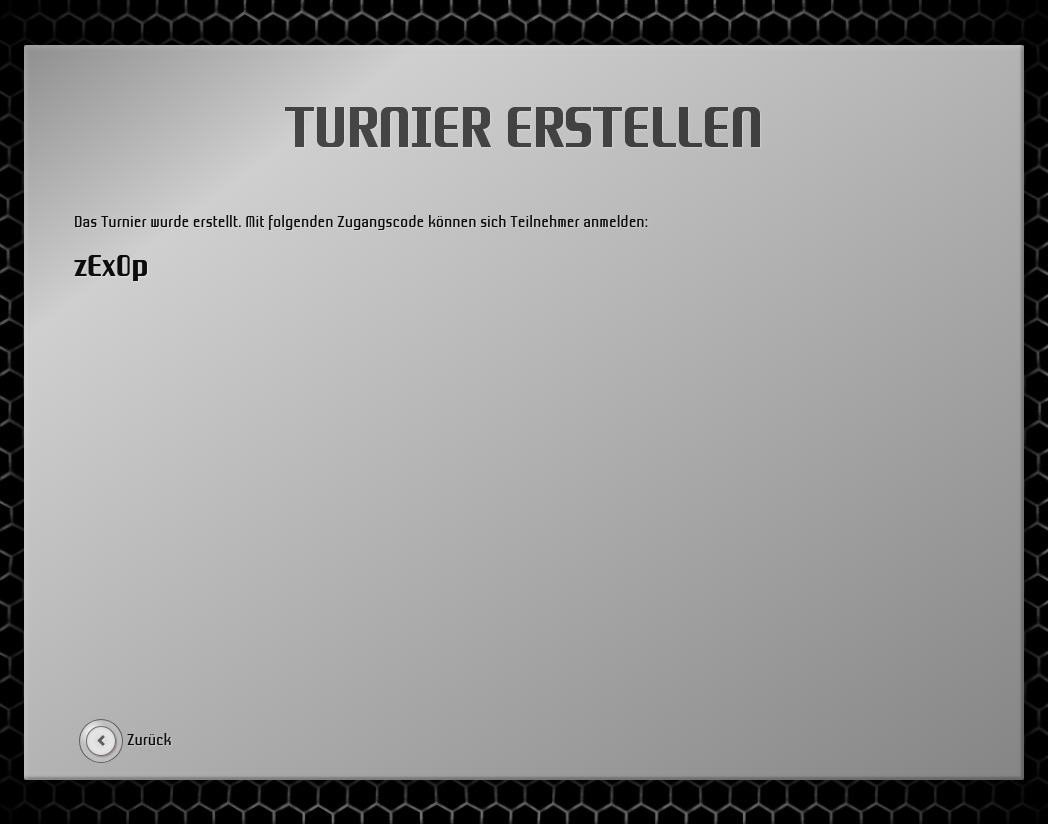
\includegraphics[width=15cm, keepaspectratio]{figures/7-turnier-erstellen-code.png}
  \caption{Der Zugangscode zum Turnier nach Erstellung des Turniers}
\end{figure}

\begin{figure}
  \centering
  \label{participate-tournament}
  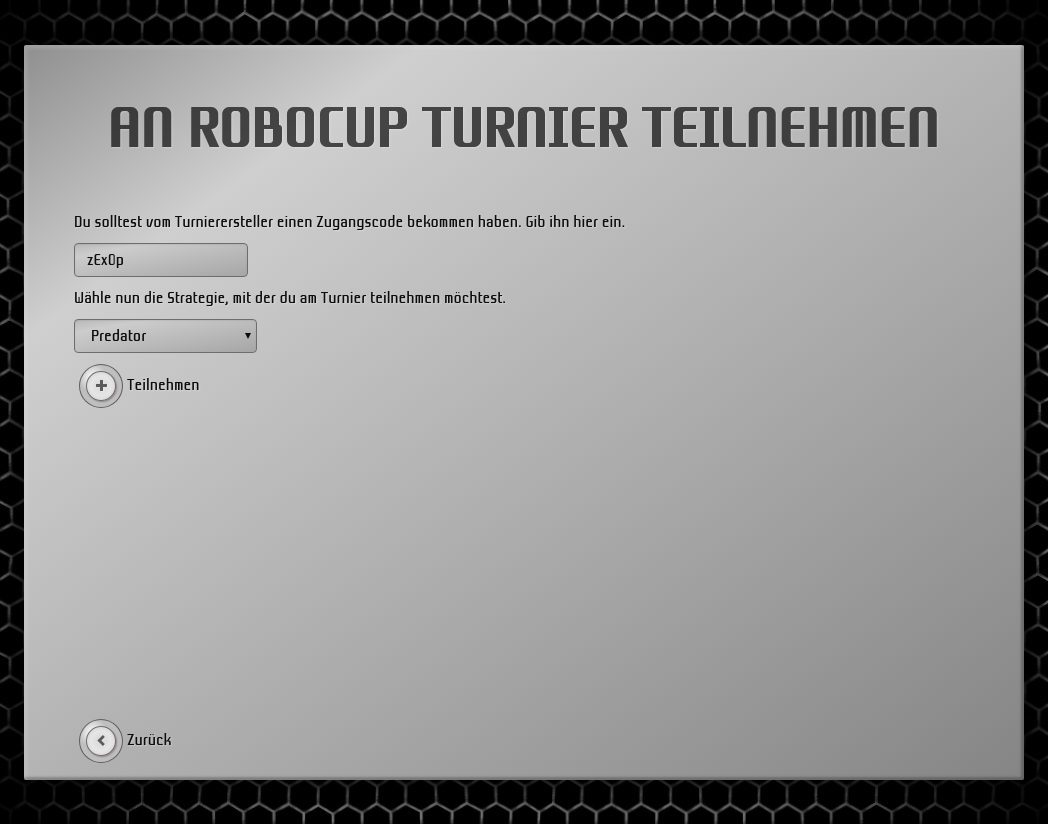
\includegraphics[width=15cm, keepaspectratio]{figures/9-turnierteilnahme.png}
  \caption{Der Dialog zur Teilnahme am Turnier}
\end{figure}

\begin{figure}
  \centering
  \label{tournament-lobby}
  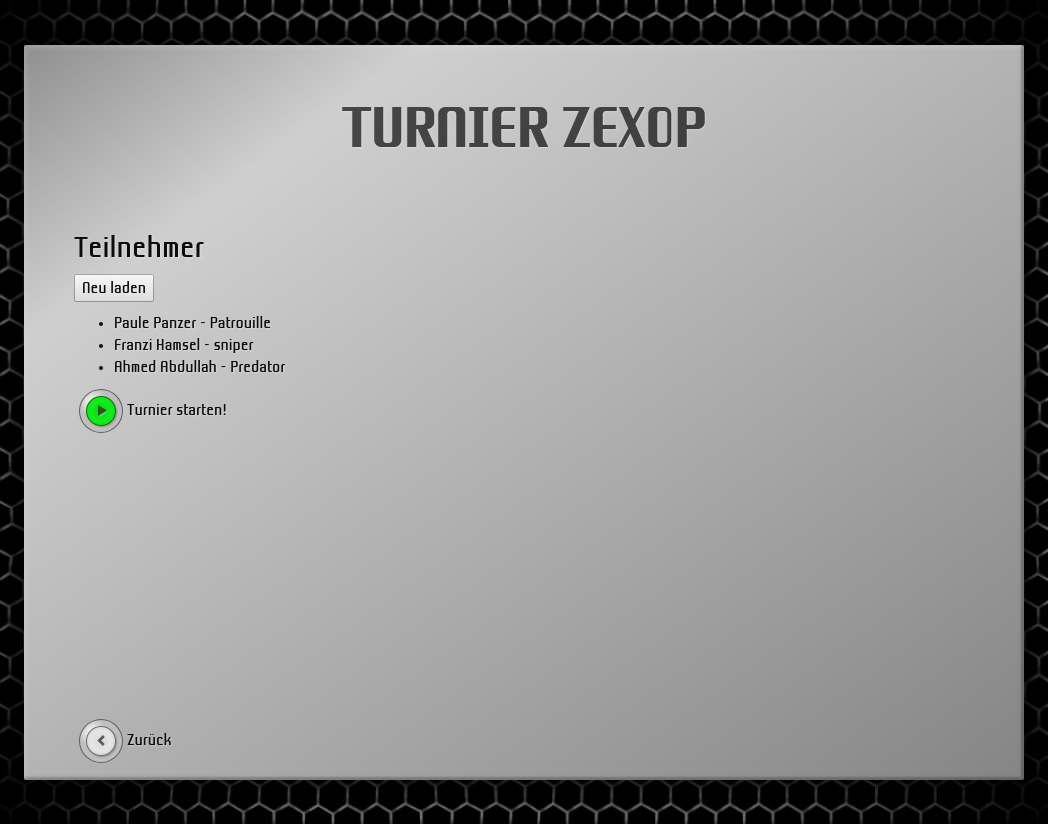
\includegraphics[width=15cm, keepaspectratio]{figures/10-turnierlobby.png}
  \caption{Die Turnierlobby}
\end{figure}

\begin{figure}
  \centering
  \label{tournament-execution-start}
  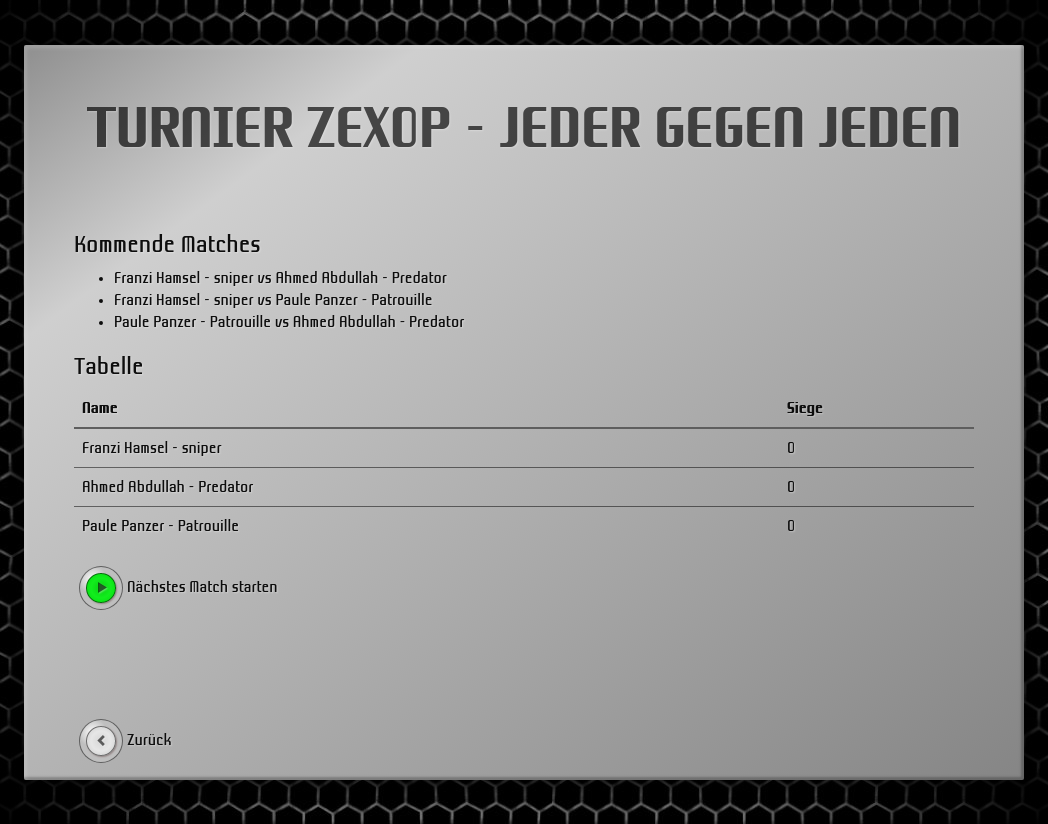
\includegraphics[width=15cm, keepaspectratio]{figures/11-turnierdurchfuehrung-start.png}
  \caption{Die Übersicht zur Turnierdurchführung im Jeder-gegen-Jeden-System zu Beginn eines Turniers}
\end{figure}

\begin{figure}
  \centering
  \label{tournament-execution-match}
  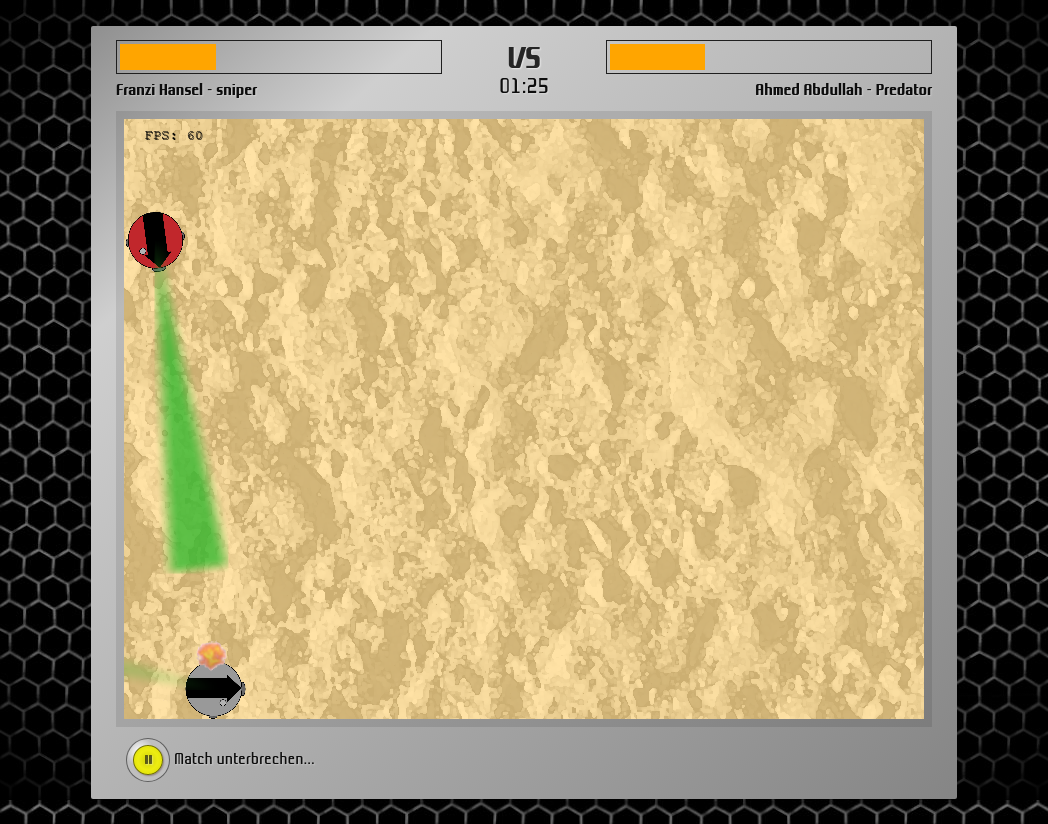
\includegraphics[width=15cm, keepaspectratio]{figures/14-turnierdurchfuehrung-kampf.png}
  \caption{Die Ansicht eines Turnierkampfes}
\end{figure}

\begin{figure}
  \centering
  \label{tournament-execution-mid}
  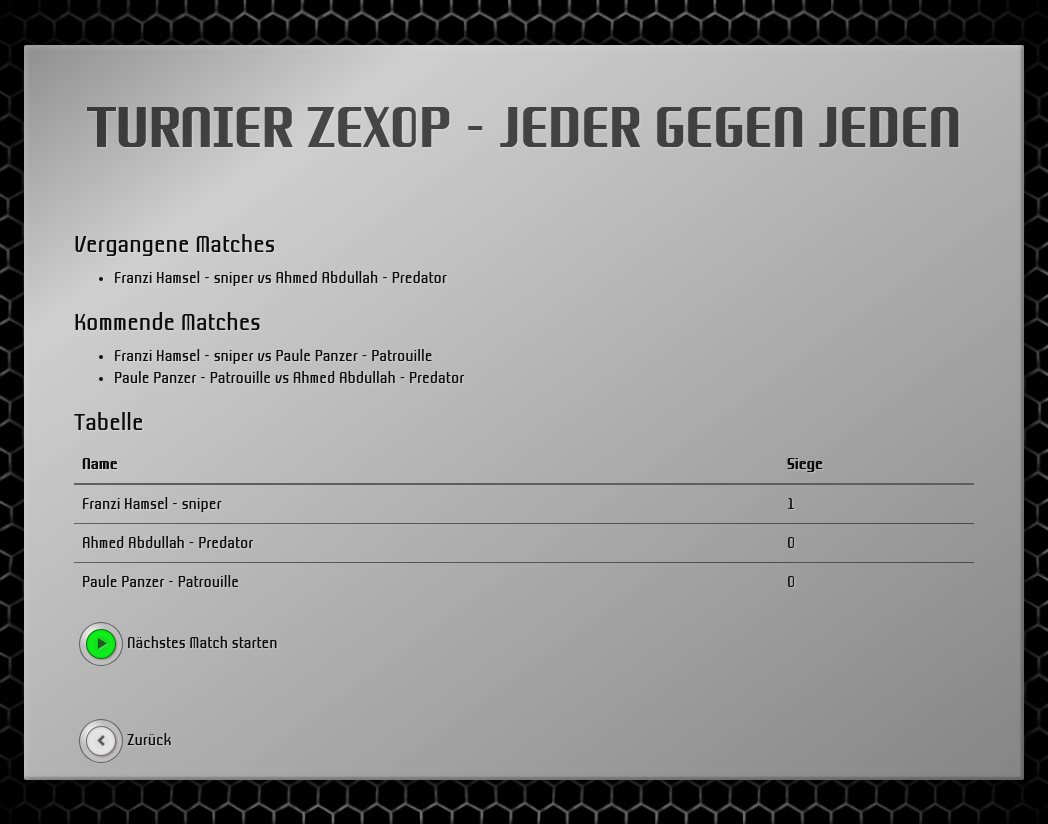
\includegraphics[width=15cm, keepaspectratio]{figures/13-turnierdurchfuehrung-mitte.png}
  \caption{Die Übersicht zur Turnierdurchführung im Jeder-gegen-Jeden-System nachdem ein Kampf durchgeführt wurde}
\end{figure}

\begin{figure}
  \centering
  \label{tournament-execution-end}
  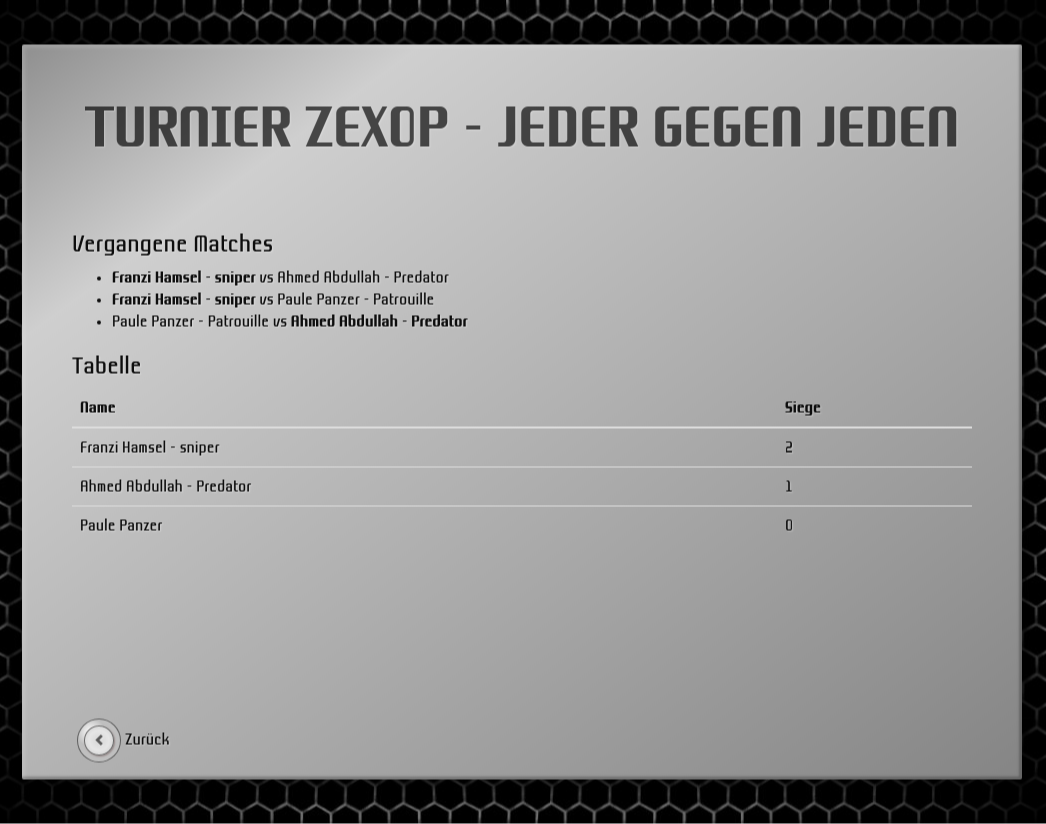
\includegraphics[width=15cm, keepaspectratio]{figures/15-turnierdurchfuehrung-ende.png}
  \caption{Die Übersicht zur Turnierdurchführung im Jeder-gegen-Jeden-System nach Ende des letzten Kampfes}
\end{figure}

\begin{figure}
  \centering
  \label{tournament-execution-ko-start}
  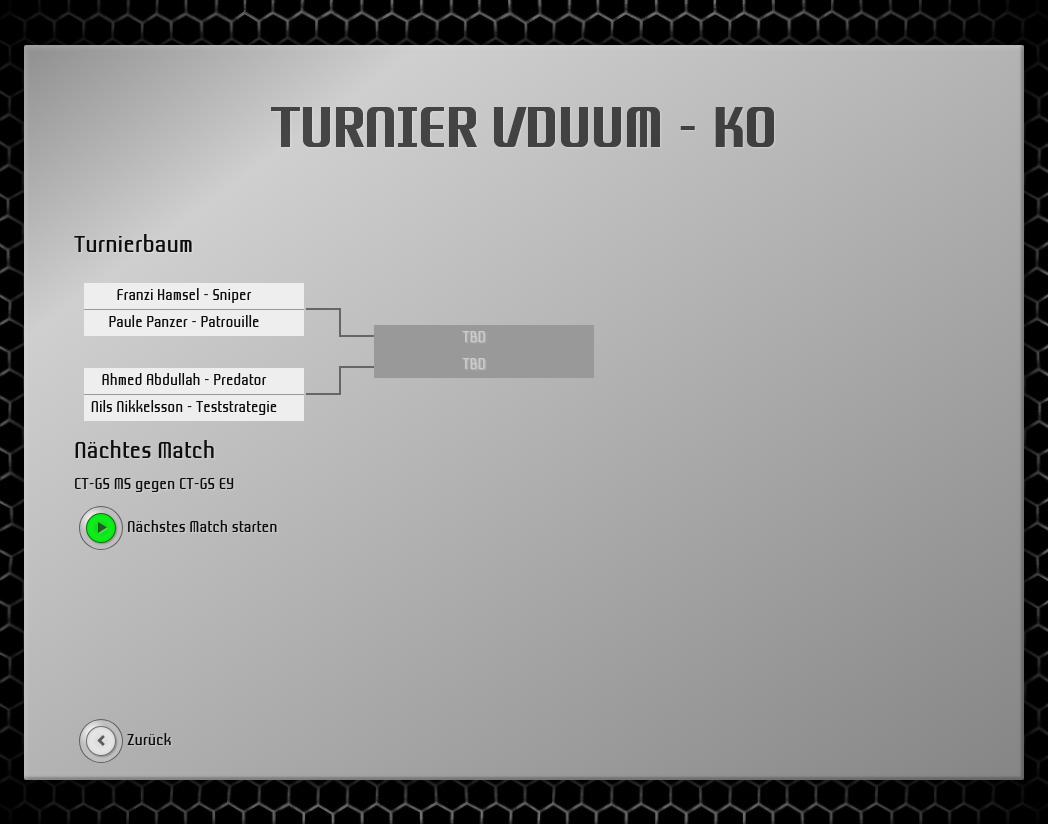
\includegraphics[width=15cm, keepaspectratio]{figures/16-turnierdurchfuehrung-ko-start.png}
  \caption{Die Übersicht zur Turnierdurchführung im KO-System bei Beginn des Turniers}
\end{figure}

\begin{figure}
  \centering
  \label{tournament-execution-ko-start}
  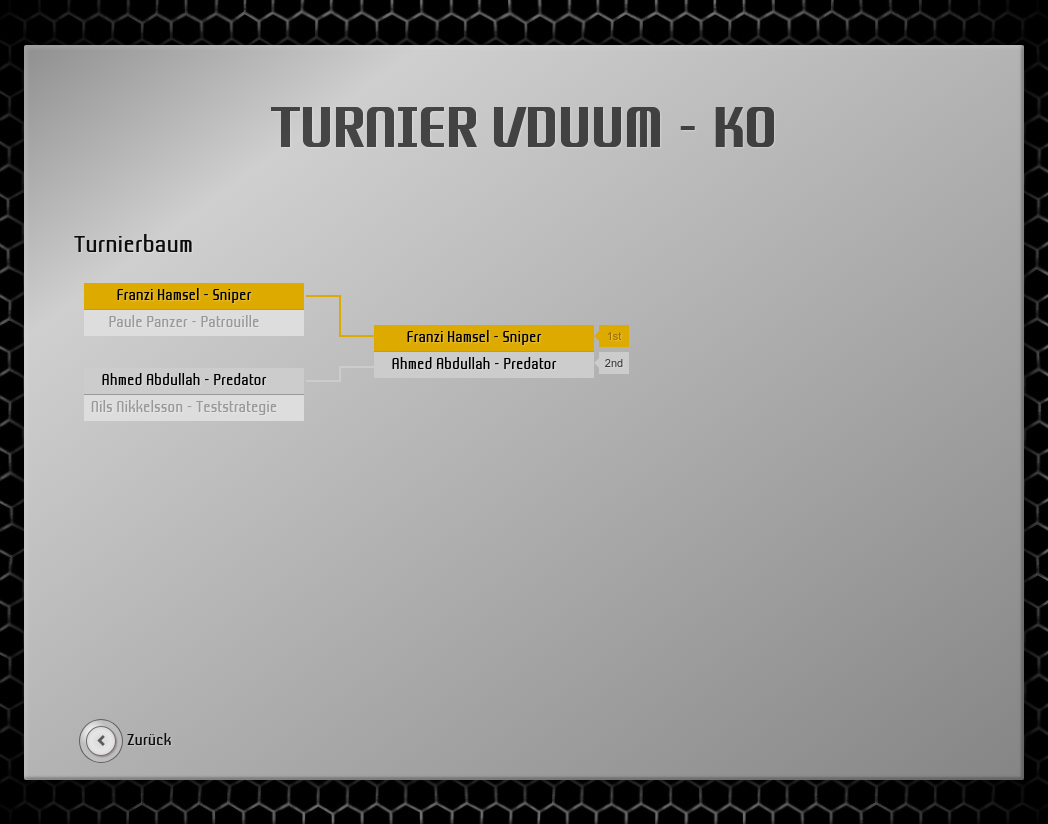
\includegraphics[width=15cm, keepaspectratio]{figures/16-turnierdurchfuehrung-ko-ende.png}
  \caption{Die Übersicht zur Turnierdurchführung im KO-System zum Ende des Turniers}
\end{figure}
